\documentclass[class=book, crop=false, oneside, 12pt]{standalone}
\usepackage{standalone}
\usepackage{amsmath}
\usepackage{../../style}
\graphicspath{{./assets/images/}}

% arara: pdflatex: { synctex: yes, shell: yes }
% arara: latexmk: { clean: partial }
\begin{document}

\chapter{Cinematica del punto}

\section{Introduzione}
La \emph{meccanica} riguarda lo studio del moto di un corpo: spiega la relazione che esiste tra le cause che generano il moto e le sue caratteristiche esprimendole con leggi quantitative.
  \subsection{Punto materiale}
  Si definisce punto materiale un \emph{corpo puntiforme privo di dimensioni}.
  \`E assimilabile a un corpo di dimensioni trascurabili rispetto a quelle dello spazio in cui si muove o degli altri corpi con cui interagisce.
  L'utilizzo di un punto materiale rende l'analisi moto pi\`u semplice in quanto \emph{rende trascurabili le propriet\`a fisiche del corpo}, come la sua forma o dimensione, ininfluenti sul moto stesso.
    Inoltre, a differenza di un corpo esteso, non pu\`o compiere rotazioni o vibrazioni.
  \subsection{Cinematica}
  Un analisi completa del moto comprende:
    \begin{itemize}
      \item il collegamento del moto alle interazioni del corpo in esame con i corpi circostanti;
      \item la descrizione geometrica dell'evoluzione temporale del fenomeno di movimento.
    \end{itemize}
  Si dice \emph{cinematica} lo studio descrittivo del moto di un corpo indipendente dalle cause che lo determinano.
    \subsubsection{Concetti fondamentali}
      \paragraph{Moto}
      Il moto di un punto materiale \`e determinato se nota la sua posizione in funzione del tempo in un determinato sistema di riferimento, sia questo cartesiano (\(x(t), y(t), z(t)\)) o polare.
      \paragraph{Traiettoria}
      La traiettoria \`e il luogo dei punti occupati successivamente dal punto in movimento.
      Costituisce pertanto una curva continua nello spazio.
      \paragraph{Grandezze fondamentali}
      \begin{itemize}
        \item Spazio: la posizione del corpo.
        \item Velocit\`a: la variazione di posizione lungo la traiettoria.
        \item Accelerazione: variazioni della velocità nel tempo.
      \end{itemize}
\section{Quiete}
La \emph{quiete} è un particolare tipo di moto in cui le coordinate restano costanti e quindi \emph{velocità e accelerazione sono nulle}.
Si noti come questo stato non \`e assoluto ma relativo al sistema di riferimento da cui si osserva il moto.
Lo stesso \emph{punto materiale} può apparire diverso in sistemi di riferimento differenti.
\section{Moto rettilineo}
Il \emph{moto rettilineo} si svolge lungo una retta sulla quale vengono fissati arbitrariamente un'origine e un verso ed è pertanto descrivibile tramite una sola coordinata \(x(t)\).
Le misure ottenute possono essere rappresentate in un sistema con due assi cartesiani detto \emph{diagramma orario}: sull'asse delle ordinate riportiamo i valori di \(x\) (metri) e su quello delle ascisse i corrispondenti valori del tempo (secondi).

  \subsection{Velocità}
    \subsubsection{Velocit\`a media}
    \begin{equation}\label{velocita_media}
      v_m = \dfrac {\Delta x} {\Delta t} = \dfrac {x_2 - x_1} {t_2 - t_1} \udm{\dfrac {m} {s}}
    \end{equation}
    \subsubsection{Velocit\`a istantanea}
    Per sopperire alla mancanza di informazioni della velocit\`a media, in modo da individuare \(x(t)\) e le sue variazioni si suddivide \(\Delta t\) in numerosi piccoli intervalli \((\Delta x)_i\) percorsi in altrettanti piccoli intervalli \((\Delta t)_i\).

    Si noti come le corrispondenti velocit\`a medie $v_i=\frac{(\Delta x)_i}{(\Delta t)_i}$ sono diverse tra di loro e da $v_m$ in quanto in un generico moto rettilineo la velocit\`a non \`e costante nel tempo.
    Suddividendo $\Delta x$ in un numero elevatissimo di intervalli $dx$ infinitamente piccoli si pu\`o definire la velocit\`a istantanea in un istante $t$ del punto in movimento come:
    \begin{equation}
      v=\lim\limits_{\Delta t\rightarrow 0}\dfrac{\Delta x}{\Delta t}=\dfrac{dx}{dt}
    \end{equation}
    La velocit\`a istantanea rappresenta pertanto la rapidit\`a di variazione temporale della posizione nell'istante $t$ considerato: pu\`o pertanto essere espressa in funzione del tempo $v(t)$.
    Il segno fa riferimento al verso del moto su $x$.
  \subsection{Accelerazione}
  La velocit\`a $v(t)$ pu\`o variare in un determinato $\Delta t$ di una quantit\`a $\delta v$.
  Questa variazione si definisce accelerazione.
  Analogamente alla velocit\`a media si definisce l'accelerazione media come:
  \begin{equation}
	a_m=\dfrac{dv}{dt}\udm{\dfrac{m}{s^2}}
  \end{equation}
  Allo stesso modo si definisce accelerazione istantanea:
  \begin{equation}
	a=\dfrac{dv}{dt}=\dfrac{d^2x}{dt^2}
  \end{equation}
    \subsubsection{Significato fisico}
    Si noti come:
    \begin{itemize}
      \item $a=0$ implica velocit\`a costante e pertanto moto rettilineo uniforme.
      \item $a>0$ implica che la velocit\`a cresce nel tempo.
      \item $a<0$ implica che la velocit\`a decresce nel tempo.
    \end{itemize}
  \subsection{Operazioni sul moto rettilineo}
    \subsubsection{Ottenere la velocit\`a nota la legge oraria}
    Nota la legge oraria $x(t)$ si pu\`o ottenere la velocit\`a istantanea con l'operazione di derivazione.
    \subsubsection{Ottenere la legge oraria nota la velocit\`a}
		Nota la dipendenza del tempo della velocit\`a istantanea $v(t)$ si pu\`o ottenere la legge oraria $x(t)$ tramite l'operazione inversa rispetto alla derivazione: l'integrazione.

		Supponendo che il punto si trovi in $x$ al tempo $t$ e nella posizione $x+dx$ in $t+dt$ da $v=\frac{dx}{dt}$ si nota come lo spostamento infinitesimo $dx$ \`e uguale al prodotto del tempo $dt$ impiegato a percorrerlo per il valore della velocit\`a al tempo $t:dx=v(t)dt$, qualunque sia la dipendenza della velocit\`a dal tempo.
		Lo spostamento complessivo sulla retta su cui si muove il punto in un intervallo finito $\Delta t = t - t_0$ \`e dato dunque dalla somma di tutti i successivi valori $dx$.
		\begin{align*}
			\Delta x &= \int_{x_0}^x dx = \int_{t_0}^t v(t)dt\\
			 x - x_0 &= \int_{t_0}^t v(t)dt\\
			       x &= x_0 +\int_{t_0}^tv(t)dt
		\end{align*}
		Si ottiene pertanto la relazione generale che permette il calcolo dello spazio percorso nel moto rettilineo:
		\begin{equation}
			x(t) = x_0 + \int_{t_0}^t v(t)dt
		\end{equation}

		\subsubsection{Relazione tra velocit\`a media e istantanea}
		Ricordando \eqref{velocita_media}, la relazione tra velocit\`a media e istantanea:
		\begin{equation*}
			v_m = \dfrac{1}{t-t_0}\int_{t_0}^{t}v(t)dt
		\end{equation*}
		\subsubsection{Ottenere la velocit\`a nota l'accelerazione}
		Data una $a(t)$ si ricava $v(t)$:
		\begin{gather*}
			dv = a(t)dt\\
			\Delta v = \int_{v_0}^v dv =\int_{t_0}^t a(t)dt
		\end{gather*}
		Pertanto:

		\begin{equation}
			v(t) = v_0 + \int_{t_0}^t a(t)dt
		\end{equation}

		\subsubsection{Dipendenza dell'accelerazione dalla posizione}
		Nota la dipendenza dell'accelerazione dalla posizione, ovvero $a(x)$ si pu\`o ricavare il valore della velocit\`a in ogni posizione $x$ o $v(x)$.
		Questo avviene considerando le funzioni di funzione.
		Se ad un istante $t$ il punto occupa una posizione $x$ con velocit\`a $v$ e accelerazione $a$ si possono pensare come funzioni della posizione e
		$$v(t) = v[x(t)]$$
		$$a(t) = a[x(t)]$$
		Derivando la prima rispetto al tempo e sfruttando la regola di derivazione delle funzioni di funzioni:
		\begin{align*}
			a[x(t)] &= \dfrac{d}{dt}v[x(t)] = \dfrac{d}{dt}\dfrac{d}{dt}\dfrac{dv}{dx}\dfrac{dx}{dt} = \dfrac{dv}{dx}\dfrac{dx}{dt}\\
			a  	    &= \dfrac{dv}{dx}\\
			adx     &= vdv
		\end{align*}
		Ovvero se dalla posizione $x$ dove un punto possiede una velocit\`a $v$ e un'accelerazione $a$ si ha uno spostamento $dx$, allora il punto subisce una variazione di velocit\`a $dv$.
		Integrando:
		\begin{align*}
			\int_{t_0}^t a(x)dx &= \int_{v_0}^{v} vdv = \dfrac{1}{2}v^2 -\dfrac{1}{2}v_0^2
		\end{align*}
		Dove $v_0$ \`e la velocit\`a in $x_0$.
		Questo permette il calcolo della variazione di velocit\`a nel passaggio dalla posizione $x_0$ a $x$.
			\paragraph{Moto uniformemente accelerato}
			Nel moto uniformemente accelerato:
			$$v^2 = v_0^2 + 2a(x-x_0)$$
\section{Moto rettilineo uniforme}
Si intende per moto rettilineo uniforme un tipo di moto rettilineo in cui la velocit\`a \`e costante.
  \subsection{Legge oraria del moto rettilineo uniforme}
	Considerando il moto rettilineo uniforme in cui $v$ \`e costante si ha:
	\begin{align*}
		x(t) &= x_0 + v\int_{t_0}^t dt=x_0 + v(t-t_0)=x_0 + vt\qquad\qquad se\ t_0 = 0
	\end{align*}
	Si nota pertanto come nel moto rettilineo uniforme lo spazio \`e una funzione lineare del tempo e la velocit\`a istantanea coincide con la velocit\`a media.
\section{Moto rettilineo uniformemente accelerato}
Si intende per moto rettilineo uniformemente accelerato un moto in cui l'accelerazione \`e costante durante il moto.
  \subsection{Dipendenza della velocit\`a dal tempo}
	La dipendenza della velocit\`a dal tempo \`e lineare:
	\begin{align*}
	  v(t) &=v_0+a(t-t_0)\\
		v(t) &=v_0+at\qquad\qquad se\ t_0 = 0
	\end{align*}
	\subsection{Dipendenza della posizione dal tempo}
	Lo spazio \`e una funzione quadratica del tempo:
	\begin{align*}
		x(t) &= x_0 +\int_{t_0}^t [v_0 + a(t-t_0)]dt= x_0 + \int_{t_0}^t v_0dt + \int_{t_0}^t a(t-t_0)dt\\
	  x(t) &= x_0 + v(t-t_0) +\dfrac{1}{2}a(t-t_0)^2= x_0 + v_0t +\dfrac{1}{2}at^2\qquad\qquad se\ t_0 = 0
	\end{align*}
\section{Moto verticale di un corpo}
Trascurando l'attrito con l'aria un corpo lasciato libero di cadere in vicinanza della superficie terrestre si muove verso il basso con una accelerazione costante $g=9.8\frac{m}{s^2}$.
Il moto \`e pertanto rettilineo uniformemente accelerato.
	\subsection{Sistema di riferimento}
	Il sistema di riferimento ha origine al suolo e l'asse delle $x$ rivolto verso l'alto.
	In questo sistema pertanto $a=-g=-9.8\frac{m}{s^2}$.
	\subsection{Caduta da un'altezza con velocit\`a iniziale nulla}
	Nel caso della caduta da un'altezza $h$ con velocit\`a iniziale nulla si nota come inizialmente:
	\begin{multicols}{3}
		\begin{itemize}
			\item $x_0 = h$.
			\item $v_0 = 0$.
			\item $t = t_0 = 0$.
		\end{itemize}
	\end{multicols}
		\subsubsection{Velocit\`a}
		Dalla dipendenza della velocit\`a dal tempo nel moto uniformemente accelerato si ottiene:
		$$v(t) = -gt$$
		E si nota come la velocit\`a aumenta in modulo durante la caduta.
		\subsubsection{Posizione}
		Osservando la dipendenza della posizione dal tempo nel moto uniformemente accelerato si ottiene:
		$$x = h -\frac{1}{2}gt^2$$
		\subsubsection{Tempo di arrivo al suolo}
		Il tempo di arrivo al suolo, dove $x=0$ \`e:
		$$t = \sqrt{\dfrac{2h}{g}}$$
		\subsubsection{Velocit\`a in funzione della posizione}
		Notando la velocit\`a in funzione della posizione nel moto uniformemente accelerato si ottiene:
		$$v^2=2g(h-x)$$
		\subsubsection{Velocit\`a di arrivo al suolo}
		Il corpo arriva al suolo con una velocit\`a:
		$$v=\sqrt{2gh}$$
	\subsection{Caduta da un'altezza con velocit\`a iniziale non nulla}
	Nel caso della caduta da un'altezza $h$ con velocit\`a iniziale non nulla si nota come inizialmente:
	\begin{multicols}{3}
		\begin{itemize}
			\item $x_0=h$.
			\item $v_0=v_i$.
			\item $t=t_0=0$.
		\end{itemize}
	\end{multicols}
		\subsubsection{Dipendenza della velocit\`a dal tempo}
		$$v(t) = -v_i -gt$$
		\subsubsection{Legge oraria}
		$$x=h-v_it-\dfrac{1}{2}gt^2$$
		\subsubsection{Dipendenza della velocit\`a dalla posizione}
		$$t(x) = \dfrac{-v_i+\sqrt{v_i^2+2g(h-x)}}{g}$$
		\subsubsection{Tempo di caduta}
		$$t_c = \dfrac{-v_i+\sqrt{v_i^2+2gh}}{g}$$
		\subsubsection{Velocit\`a di caduta}
		$$v_c^2=v_i^2+2gh$$
	\subsection{Lancio del punto verso l'alto partendo dal suolo}
	Nel caso di un lancio del punto verso l'alto si nota come inizialmente:
	\begin{multicols}{3}
		\begin{itemize}
			\item $x_0=0$.
			\item $v_0 = v_2 > 0$.
			\item $t=t_0=0$.
		\end{itemize}
	\end{multicols}
		\subsubsection{Velocit\`a}
		$$v=v_2 - gt$$
		\subsubsection{Legge oraria}
		$$x = v_2t-\dfrac{1}{2}gt^2$$
		\subsubsection{Punto pi\`u alto}
		Il punto raggiunge la posizione pi\`u alta al tempo:
		$$t_M = \dfrac{v_2}{g}$$
		E nella posizione:
		$$x_M=x(t_M)=\dfrac{v_2^2}{2g}$$
		\subsubsection{Discesa}
		Per $t\ge t_M$ si \`e nella situazione del primo esempio: punto che cade da un'altezza $x_M$ con velocit\`a iniziale nulla.
		Pertanto:
		$$t_s = \frac{\sqrt{2x_M}}{g}=t_M$$
		E la durata complessiva del moto \`e pertanto:
		$$2t_M = \dfrac{2v_2}{g}$$
		Ricavando $t(x)$ dalla legge oraria e da $v(x)$ si ha:
		\begin{align*}
			t(x) &= \dfrac{v_2\pm \sqrt{v_2^2 - 2gx}}{g}\\
			     &= t_M \pm \sqrt{t_M^2 - \dfrac{2x}{g}}\\
			v(x) &= \pm \sqrt{v_2^2 - 2gx}
		\end{align*}
\section{Moto armonico semplice}
Il moto armonico semplice lungo un asse rettilineo \`e un moto vario la cui legge oraria \`e data dalla relazione:
$$x(t) = A \sin(\omega t + \phi)$$
Dove:
\begin{multicols}{2}
	\begin{itemize}
		\item $A$ ampiezza del moto.
		\item $\omega t + \phi$ fase del moto.
		\item $\omega$ pulsazione.
		\item $\phi$ fase iniziale.
	\end{itemize}
\end{multicols}
	\subsection{Caratteristiche}
	Essendo i valori estremi della funzione seno $+1$ e $-1$ il punto percorre un segmento di ampiezza $2A$ con centro nell'origine, con uno spostamento massimo da essa $A$.
	Al tempo $t=0$ occupa $x(0)=A\sin\phi$.
	Date le costanti $A$ e $\phi$ si determina la posizione iniziale del punto, che si trova a $t=0$ nell'origine solo se $\phi=\{0, \pi\}$.
	\subsection{Periodicit\`a}
	Essendo la funzione seno periodica con periodo $2\pi$ il moto risulta periodico e descrive oscillazioni di ampiezza $A$ rispetto al centro $O$ uguali tra loro e caratterizzate da una durata $T$ periodo del moto armonico.
	Si dice pertanto periodico un moto in cui in intervalli di tempo uguali il punto ripassa nella stessa posizione con la stessa velocit\`a.
	\subsection{Determinare il periodo}
	Per determinare il periodo $T$ si considerino due tempi $t$ e $t'$ tali che $t'-t = T$.
	Per definizione $x(t')=x(t)$, pertanto dalla legge oraria le fasi nei due istanti devono differire $2\pi$.
	Si ha pertanto $\omega t' +\phi = \omega t + \phi + 2\pi$, ne segue che:
	\begin{align*}
		T &= \dfrac{2\pi}{\omega}\\
		\omega &=\dfrac{2\pi}{T}
	\end{align*}
		\subsubsection{Significato di $\omega$}
		Si nota pertanto come il moto si ripeta velocemente quando la pulsazione \`e grande mentre come il moto sia lento per bassi valori della pulsazione.
		\subsubsection{Frequenza del moto}
		Si definisce frequenza $v$ del moto il numero di oscillazioni in un secondo:
		\begin{align*}
			v &= \dfrac{1}{T}\\
			  &= \dfrac{\omega}{2\pi}\\
			\omega &= 2\pi v
		\end{align*}
		Si noti come il periodo e la frequenza di un moto armonico sono indipendenti dall'ampiezza del moto.
		\subsubsection{Classi di moti armonici}
		Fissato il valore della pulsazione si ottiene una classe di moti armonici caratterizzata dallo stesso periodo che differiscono tra loro per i diversi valori dell'ampiezza e della fase iniziale, ovvero per le condizioni iniziali.
	\subsection{Velocit\`a}
	La velocit\`a del punto che si muove con moto armonico si ottiene derivando $x(t)$.
	\begin{align*}
		\dot{x} &= v(t) = \dfrac{dx}{dt}\\
		  &=\omega A \cos(\omega t+\phi)\\
	\end{align*}
	La velocit\`a assume il valore massimo nel centro di oscillazione dove vale $\omega A$ e si annulla agli estremi dove si inverte il senso del moto.
	\subsection{Accelerazione}
	L'accelerazione del punto che si muove con moto armonico si ottiene derivando $v(t)$.
	\begin{align*}
		\ddot{x} = a(t) = \dfrac{dv}{dt} = \dfrac{d^2x}{dt^2}= -\omega^2 A \sin(\omega t + \phi)= -\omega^2 x
	\end{align*}
	L'accelerazione si annulla nel centro di oscillazione e assume il valore in modulo massimo $\omega^2 A$ agli estremi, dove si inverte la velocit\`a.
	Si nota inoltre come sia proposizionale ed opposta allo spostamento dal centro di oscillazione.
	A parte il valore dell'ampiezza, le tre funzioni mostrano lo stesso andamento temporale; si nota unicamente uno spostamento di una rispetto all'altra lungo l'asse dei tempi.
	
	Si nota pertanto come la velocit\`a sia sfasata di $\frac{\pi}{2}$  rispetto allo spostamento o si trova in quadratura di fase, mentre l'accelerazione \`e sfasata di $\pi$ rispetto allo spostamento o si trova in opposizione di fase.
	\subsection{Condizioni iniziali}
	Le costanti $A$ e $\phi$ identificano le condizioni iniziali:
	$$ x(0) = x_0 = A \sin\phi$$
	$$v(0) = v_0 = \omega A \cos\phi$$
	Note le condizioni iniziali $x_0$ e $v_0$ si calcolano $A$ e $\phi$ come:
	$$\tan \phi = \dfrac{\omega x_0}{v_0}$$
	$$A^2 = x_0^2 + \dfrac{v_0^2}{\omega^2}$$
	\subsection{Dipendenza della velocit\`a dalla posizione}
	\begin{align*}
		v(x) &= \int_{x_o}^x a(x)dx=-\omega^2\int_{x_0}^x xdx=\dfrac{1}{2}\omega^2(x_x^2-x^2)=\dfrac{1}{2}v^2 - \dfrac{1}{2}v_0^2
	\end{align*}
	Pertanto
	$$v^2 = v_0^2 + \omega^2(x_0^2(x_0^2-x^2))$$
	Con riferimento al centro dove $x_0 = 0$ e $v_0 = \omega A$
	$$v^2(x)=\omega^2(A^2 - x^2)$$
	Il segno di $v$ dipende dal verso di passaggio.
	Si nota pertanto come l'accelerazione \`e proporzionale allo spostamento con segno negativo $a =-\omega^2 x$.
	\subsection{Condizione sufficiente per un moto armonico semplice}
	Se si trova che in un moto l'accelerazione \`e proporzionale allo spostamento con costante di proporzionalit\`a negativa si dimostra che quel moto \`e armonico semplice.
	La condizione necessaria e sufficiente affinch\`e un moto sia armonico \`e:
	$$\dfrac{d^2x}{dt^2}+\omega^2x=0$$
	O equazione differenziale del moto armonico.
	Le funzioni seno e coseno e le loro combinazioni lineari sono tutte e sole le funzioni che soddisfano la condizione nel campo reale.
		\subsubsection{Moto con funzione coseno}
		Queste considerazioni portano a considerare una legge del moto che utilizzi la funzione coseno.
		Si noti come le due funzioni differiscono per un termine di sfasamento $\frac{\pi}{2}$.
		Ovvero $x=A\sin(\omega t+\phi)$ e $x = A\cos(\omega t+\phi)$ rappresentano lo stesso moto, solo che il primo \`e visto a partire dall'istante $t_0$, mentre il secondo dall'istante $t_0 + \dfrac{T}{4}$.
	\subsection{Oscillazione}
	Se in un diverso fenomeno fisico si trova una grandezza $f$ che obbedisce a
	$$\dfrac{d^2f}{dz^2}+k^2f=0$$
	La soluzione \`e sempre:
	$$f(z)=A\sin(kz+\phi)$$
	Ovvero $f$ descrive un'oscillazione rispetto a $z$ il cui periodo dipende da $k$.
\section{Moto rettilineo smorzato esponenzialmente}
Si consideri ora un altro moto vario in cui l'accelerazione soddisfa la condizione $a = -kv$, con $k$ costante positiva.
L'accelerazione \`e sempre contraria alla velocit\`a che deve necessariamente diminuire e varia con la stessa legge con cui varia la velocit\`a, ovvero:
$$a = \dfrac{dv}{dt} = -kv$$
Integrando con il metodo della separazione delle variabili:
\begin{align*}
	&\dfrac{dv}{v} = -kdt\\
	\Rightarrow&\int_{v_0}^v\dfrac{dv}{v} = -k\int_0^t\\
	\Rightarrow &\log\dfrac{v}{v_0} = -kt
\end{align*}
Dove $v_0$ \`e la velocit\`a in $t=0$ e $v_0\neq 0$.
Passando alle esponenziali:
$$v(t) = v_0e^{-kt}$$
La velocit\`a decresce esponenzialmente nel tempo e il punto alla fine si ferma.
	\subsection{Cambio della velocit\`a con la posizione}
	\begin{align*}
		&a = \dfrac{dv}{dt}=\dfrac{dv}{dx}\dfrac{dx}{dt}=\dfrac{dv}{dx}v = -kv\Rightarrow\\
		&\Rightarrow \dfrac{dv}{dx}=-k\Rightarrow\\
		&\Rightarrow dv = -kdx\Rightarrow\\
		&\Rightarrow \int_{v_0}^v dv = -k \int_0^xdx\\
	\end{align*}
	Risulta pertanto un andamento lineare decrescente
	$$v(x)=v_0-kx$$
	La velocit\`a si annulla in
	$$x=\dfrac{v_0}{k}$$
	dove il punto si ferma.
	\subsection{Legge oraria}
	La legge oraria si ricava per integrazione da $v(t)$:
	\begin{align*}
		x(t)=x_0+\int_0^t v(t)dt=\int_0^tv_0e^{-kt}dt=-\dfrac{v_0}{k}[e^{-kt}]_0^t=\dfrac{v_0}{k}(1-e^kt)
	\end{align*}
	\subsection{Costante di tempo}
	La rapidità di variazione della funzione $e^{-kt}$ è determinata dal valore di $k$.
	Posto
	$$\tau = \dfrac{1}{k}$$
	detto anche \emph{costante di tempo}, so che in un intervallo di tempo pari a $\tau$ la funzione si riduce di un fattore di $e$
	$$\frac{e^{-k\left(t + \tau\right)}}{e^{-k \tau}} = e^{-1}$$
	Minore il valore di $\tau$ pi\`u rapida la decrescita.

\section{Moto nel piano}
  \subsection{Posizione}
  Nel caso che il moto sia vincolato a svolgersi su di un piano la traiettoria del punto $P$ è in generale  una linea curva.
  Si devono quindi analizzare la direzione e verso del moto oltre al valore numerico dello spostamento.
  Grandezze con queste caratteristiche si chiamano \emph{vettori}.

  Si definisce vettore un segmento orientato caratterizzato da un \emph{modulo}, una \emph{direzione} ed un \emph{verso}.
    \subsubsection{Determinare un punto nel piano}
    Un punto nel piano \`e individuato da due coordinate distinte che possono fare riferimento a un sistema di coordinate cartesiane o polari.
    Questi due sistemi sono messi in relazione secondo:
    \begin{equation}
      x = r \cos \theta \ , \ y = r \sin \theta
    \end{equation}
    \begin{equation}
      r = \sqrt{x^2 + y^2 } \ , \ \tan \theta = \frac{y}{x}
    \end{equation}
    \subsubsection{Raggio vettore}
    La posizione del punto \(P\) può anche essere individuata per mezzo del \emph{raggio vettore} (segmento che va dall'origine \(O\) fino al punto \(P\)):
    \begin{equation}
      \overrightarrow{r}(t) = OP = x(t) \overrightarrow{u}_x + y(t) \overrightarrow{u}_y
    \end{equation}
    Dove \(\overrightarrow{u}_x\) e \(\overrightarrow{u}_y\) rappresentano i versori degli assi cartesiani che si considerano fissi nel tempo.
    Se è nota la dipendenza dal tempo di \(\overrightarrow{r}\), cioè la funzione \(\overrightarrow{r}(t)\), è individuato il moto del punto \(P\).
    \subsubsection{Coordinata curvilinea}
    La posizione del punto lungo la traiettoria può anche essere data da una coordinata curvilinea \(s\) (direzione tangente punto per punto), misurata a partire da un'origine arbitraria.
    Il valore di \(s\) esprime la lunghezza della traiettoria e varia nel tempo durante il moto: \(\frac{ds}{dt}\) indica la variazione temporale della posizione lungo la traiettoria cioè la velocità istantanea del punto, come definita nel modo rettilineo.
    Se diamo la forma della traiettoria e la velocità con cui viene percorsa abbiamo fornito una descrizione completa del moto.
  \subsection{Velocit\`a vettoriale}
  Considerando due posizioni occupate dal punto \(P\) al tempo \(t\) e al tempo \(t + \Delta t\): esse sono individuate dai vettori \(\overrightarrow{r}(t)\) e \(\overrightarrow{r}(t + \Delta t) = \overrightarrow{r}(t) + \Delta \overrightarrow{r}\).
  Si costruisce il rapporto incrementale \(\frac{\overrightarrow{r}(t+\Delta t) - \overrightarrow{r}(t)}{\Delta t} = \frac{\Delta \overrightarrow{r}}{\Delta t}\) e si definisce velocità vettoriale il limite per \(\Delta t \rightarrow 0\):
  \begin{equation*}
    v = \lim\limits_{\Delta t \rightarrow 0} \dfrac{\Delta\overrightarrow{r}}{\Delta t}= \dfrac{d \overrightarrow{r}}{dt}
  \end{equation*}
  La velocità vettoriale è pertanto la derivata del raggio vettore rispetto al tempo.
  Al limite l'incremento del raggio vettore risulta in direzione tangente alla traiettoria nel punto \(P\) e in modulo e uguale allo spostamento infinitesimo \(ds\) lungo la traiettoria,
  per cui possiamo scrivere \(d \overrightarrow{r} = ds \overrightarrow{u}_T\) dove \(\overrightarrow{u}_t\) è il versore della tangente alla curva, variabile nel tempo man mano che il punto avanza lungo la traiettoria.
  Questo non vale se non si è all'infinitesimo, lo si vede chiaramente con spostamenti \(\Delta s\) più grandi.
  In sostanza si considera il moto come una successione di spostamenti rettilinei infinitesimi con direzione variabile: la direzione istantanea del moto coincide con quella della tangente alla traiettoria nel punto occupato all'istante considerato.
  \begin{equation*}
    \overrightarrow{v} = \frac{ds}{dt} \overrightarrow{u}_T = v \overrightarrow{u}_T
  \end{equation*}
  Pertanto la velocità vettoriale \(\overrightarrow{v}\) individua in ogni istante con la sua direzione e verso il suo moto e con il suo modulo \(v = \frac{ds}{dt}\) la velocità istantanea con cui è percorsa la traiettoria.

  Bisogna fare attenzione a non confondere i concetti di raggio vettore e i suoi incrementi finiti da una parte e il percorso effettivo dall'altra: un punto potrebbe percorrere un'orbita chiusa ritornando al punto di partenza e in tal caso il raggio vettore non cambia, ma il punto ha percorso una traiettoria finita (\(\Delta \overrightarrow{r} = 0, \Delta s \neq 0\)) con velocità vettoriale istantanea diversa da zero (similmente a quello che accadeva nel MRU, risulta nulla la velocità vettoriale media).

  La traiettoria del moto e la definizione di velocità \(v = \overrightarrow{u}_T\) non dipendono dal sistema di riferimento (invarianza delle relazioni vettoriali rispetto alla scelta del sistema di riferimento).
  Tuttavia un vettore che si esprime esplicitamente tramite le sue componenti cambia perciò queste dipendono dal sistema di riferimento.
		\subsubsection{Calcolo delle componenti della velocit\`a}
			\paragraph{Componenti cartesiane}
      Essendo $\overrightarrow{r}=x\overrightarrow{u_x}+y\overrightarrow{u_y}$,
			\begin{align*}
        v =\dfrac{d\overrightarrow{r}}{dt}
          =\dfrac{dx}{dt}\overrightarrow{u_x}+\dfrac{dy}{dt}\overrightarrow{u_y}
          =v_x\overrightarrow{u_x} + v_y\overrightarrow{u_y}
			\end{align*}
			La velocit\`a del punto $P$ ha componenti cartesiani $v_x$ e $v_y$ dei due moti rettilinei descritti dai punti proiezione di $P$ sugli assi cartesiani.
			Pertanto
			$$v=\sqrt{v^2_x+v_y^2}$$
			Inoltre detto $\phi$ l'angolo tra il vettore $v$ e l'asse $x$,
			$$\tan\phi = \dfrac{v_y}{v_x}$$
			\paragraph{Componenti polari}
      Introducendo $\overrightarrow{u_r}$ e $\overrightarrow{u_\theta}$, il versore della direzione di $\overrightarrow{r}$ e il versore ortogonale alla stessa, si nota come questi cambiano direzione durante il moto.
      Il raggio vettore $\overrightarrow{r}$ pu\`o essere espresso come $ru_r$, pertanto:
			\begin{align*}
        v&=\dfrac{d\overrightarrow{r}}{dt}=\dfrac{d\overrightarrow{r}}{dt}\overrightarrow{u_r}+r\dfrac{d\overrightarrow{u_r}}{dt}\Rightarrow\\
        v&=\dfrac{d\overrightarrow{r}}{dt}\overrightarrow{u_r}+r\dfrac{d\theta}{dt}\overrightarrow{u_\theta}=v_r+v_\theta\\
			\end{align*}
      La velocit\`a, sempre tangente alla traiettoria si scompone in due componenti: la velocit\`a radiale $v_r$ diretta lungo $\overrightarrow{r}$ e di modulo $\frac{dr}{dt}$ e la velocit\`a trasversa $v_\theta$ ortogonale a $\overrightarrow{r}$ e di modulo $r\frac{d\theta}{dt}$.
			$v_r$ dipende dalle variazioni del modulo del raggio vettore $v_\theta$, collegata alle variazioni di direzione dello stesso.
			Il modulo della velocit\`a \`e pertanto, per queste componenti:
      $$v=\dfrac{ds}{dt}=\sqrt{\biggl(\dfrac{d\overrightarrow{r}}{dt}\biggr)^2+\overrightarrow{r}^2\biggl(\dfrac{d\theta}{dt}\biggr)^2}$$
		\subsubsection{Determinare la posizione nota la velocit\`a}
    Essendo $v=\frac{d\overrightarrow{r}}{dt}$, per ricavare la posizione da essa si integra:
    $$\overrightarrow{r}(t)=\overrightarrow{r}(t_0)+\int_{t_0}^tv(t)dt$$
		L'integrazione esplicita pu\`o essere fatta ricorrendo alle componenti, applicando
		$$x(t)=x_0+\int_{t_0}^tv(t)dt$$
		ai moti rettilinei componenti.
  \subsection{Accelerazione nel moto piano}
  L'accelerazione nel moto piano deve esprimere le variazioni della velocità sia come \emph{modulo} che \emph{direzione} e quindi ci aspettiamo che abbia due componenti,
  una legata alla variazione del modulo della velocità e la seconda al cambiamento di direzione del moto.
  Nel moto rettilineo, dove la velocità mantiene sempre la stessa direzione, l'accelerazione è espressa da un solo termine.

  Anche nel moto piano l'accelerazione si definisce come derivata della velocità rispetto al tempo (ed è una grandezza vettoriale):
  \begin{equation*}
   \overrightarrow{a} = \frac{d \overrightarrow{v}}{dt} = \frac{d^2 \overrightarrow{r}}{dt^2}
  \end{equation*}
  Derivando le componenti del vettore:
  \begin{align*}
    \overrightarrow{a}&=\frac{d}{d t}\left(v \overrightarrow{u}_{\mathrm{T}}\right)=\\
                      &=\frac{d v}{d t} \overrightarrow{u}_{\mathrm{T}}+v \frac{d \overrightarrow{u}_{\mathrm{T}}}{d t}=\\
                      &=\frac{d v}{d t} \overrightarrow{u}_{\mathrm{T}}+v \frac{d \phi}{d t} \overrightarrow{u}_{\mathrm{N}}
  \end{align*}
  La prima componente, parallela alla velocità, esprime la variazione del modulo della velocità; il secondo termine, dipendente dalla variazione di direzione della velocità, è ortogonale a questa: \(\overrightarrow{u}_N\) è un vettore ortogonale a \(\overrightarrow{u}_T\) diretto verso la concavità della traiettoria, e \(d \phi/dt \) dice quanto rapidamente cambia la direzione di \(\overrightarrow{u}_T\)  e quindi di \(\overrightarrow{u}_N\).

  Le due componenti dell'accelerazione si chiamano accelerazione tangenziale e accelerazione normale o centripeta.
  In un moto curvilineo vario entrambe le componenti sono diverse da zero; se però il moto curvilineo è uniforme è nulla \(\overrightarrow{a}_T\); se invece il moto è rettilineo vario è nulla \(\overrightarrow{a}_N\) e solo nel moto rettilineo uniforme \(\overrightarrow{a}_N\) = \(\overrightarrow{a}_T\) = \(\overrightarrow{0}\).
  In altre parole con \(a_T \neq 0\) il moto è sempre vario, con \(a_N \neq 0\) è  sempre curvilineo.
		\subsubsection{Componente normale}
			Per esprimere la componente normale, si nota come al limite per $\Delta t\rightarrow 0$ le rette normali alla traiettoria in due punti molto vicini si incontrano in $C$ che coincide con il centro della circonferenza tangente alla traiettoria in $P$, o circonferenza osculatrice.
			Questo punto si chiama centro di curvatura della traiettoria nel punto $P$.
			L'arco di traiettoria $ds$ \`e pari a $Rd\phi$ con $R=CP$ raggio di curvatura.
			Al variare di $P$ lungo la traiettoria sia $R$ che $X$ variano.
			Si nota:
			$$\dfrac{d\phi}{dt}=\dfrac{d\phi}{ds}\dfrac{ds}{dt}=\dfrac{1}{R}v$$
			Sostituendo nell'espressione dell'accelerazione trovata prima:
      $$\overrightarrow{a}=\dfrac{dv}{dt}\overrightarrow{u_T}+\dfrac{v^2}{R}\overrightarrow{u_N}=\overrightarrow{a_T}+\overrightarrow{a_N}$$
			Il modulo pertanto vale:
      $$a=\sqrt{a^2_T+a^2_N}=\sqrt{\biggl(\dfrac{d\overrightarrow{v}}{dt}\biggr)^2+\dfrac{v^4}{R^2}}$$
			Le due componenti si chiamano accelerazione tangenziale e accelerazione normale o centripeta.
		\subsubsection{Moto curvilineo uniforme}
    In un moto curvilineo vario entrambe le componenti sono diverse da zero; il moto \`e curvilineo uniforme se $\overrightarrow{a_T}$ \`e nulla, rettilineo vario se \`e nulla $\overrightarrow{a_N}$ o altrimenti rettilineo uniforme se sono entrambe nulle.
		Ovvero:
		\begin{multicols}{2}
			\begin{itemize}
        \item $\overrightarrow{a_T}\neq 0$ moto vario.
        \item $\overrightarrow{a_N}\neq 0$ moto curvilineo.
			\end{itemize}
		\end{multicols}
		\subsubsection{Componenti cartesiane}
		Le componenti cartesiane dell'accelerazione sono le accelerazioni dei due moti rettilinei proiezioni sugli assi del moto di $P$ lungo la traiettoria curva:
		\begin{align*}
      \overrightarrow{a}=\dfrac{d\overrightarrow{v}}{dt}=\dfrac{d\overrightarrow{v_x}}{dt}\overrightarrow{u_x}+\dfrac{d\overrightarrow{v_y}}{dt+\overrightarrow{u_y}}=\dfrac{d^2x}{dt^2}\overrightarrow{u_x}+\dfrac{d^2y}{dt^2}\overrightarrow{u_y}=a_x\overrightarrow{u_x}+a_y\overrightarrow{u_y}
		\end{align*}
    Detto $\phi$ l'angolo che $\overrightarrow{u_T}$ forma con $\overrightarrow{u_x}$, si deduce che:
    $$\overrightarrow{a_x}=\dfrac{d\overrightarrow{v}}{dt}\cos\phi - \dfrac{\overrightarrow{v}^2}{R}\sin\phi$$
    $$\overrightarrow{a_y}=\dfrac{d\overrightarrow{v}}{dt}\sin\phi - \dfrac{\overrightarrow{v}^2}{R}\cos\phi$$
		Dalle componenti tangenziale e centripeta si ricavano le cartesiano risolvendo il sistema lineare nelle incognite $\frac{dv}{dt}$ e $\frac{v^2}{R}$.
		\subsubsection{Componenti polari}
    Considerando che $\overrightarrow{u_r}$ e $\overrightarrow{u_\theta}$ non sono fissi e $\overrightarrow{v}=\frac{d\overrightarrow{r}}{dt}\overrightarrow{u_r}+\frac{d\theta}{t}\overrightarrow{u_\theta}$
		\begin{align*}
      \overrightarrow{a}=\dfrac{d\overrightarrow{v}}{dt}=\dfrac{d}{t}\biggl(\dfrac{d\overrightarrow{r}}{d\overrightarrow{r}}\overrightarrow{u_r}+r\dfrac{d\theta}{dt}\overrightarrow{u_\theta}\biggr)=\dfrac{d^2\overrightarrow{r}}{dt^2}\overrightarrow{u_r}+\dfrac{d\overrightarrow{r}}{dt}\dfrac{d\overrightarrow{u_r}}{dt}+\dfrac{d\overrightarrow{r}}{dt}\dfrac{d\theta}{dt}\overrightarrow{u_\theta}+r\dfrac{d^2\theta}{dt^2}\overrightarrow{u_\theta}+\overrightarrow{r}\dfrac{d\theta}{dt}\dfrac{d\overrightarrow{r_\theta}}{dt}
		\end{align*}
    Considerando che $\frac{d\overrightarrow{u_r}}{dt}=\frac{d\theta}{dt}\overrightarrow{u_\theta}$ e che $\frac{d\overrightarrow{u_\theta}}{dt}=-\frac{d\theta}{dt}\overrightarrow{u_r}$ si nota che per una variazione positiva di $\theta$ $d\overrightarrow{u_\theta}$ \`e opposto a $\overrightarrow{u_r}$  e si ha:
    $$\overrightarrow{a}=\biggl[\dfrac{d^2\overrightarrow{r}}{dt^2}-r\biggl(\dfrac{d\theta}{dt}\biggr)^2\biggr]\overrightarrow{u_r}+\biggl[2\dfrac{d\overrightarrow{r}}{dt}\dfrac{d\theta}{dt}+\overrightarrow{r}\dfrac{d^2\theta}{dt^2}\biggr]\overrightarrow{u_\theta}$$
		Da cui:
    $$\overrightarrow{a}=\biggl[\dfrac{d^2\overrightarrow{r}}{dt^2}-r\biggl(\dfrac{d\theta}{dt}\biggr)^2\biggr]\overrightarrow{u_r}+\biggl[\dfrac{1}{r}\dfrac{d}{dt}\biggl(\overrightarrow{r}^2\dfrac{d\theta}{dt}\biggr)\biggr]\overrightarrow{u_\theta}$$
		Il primo termine rappresenta l'accelerazione radiale e il secondo l'accelerazione trasversa.
    Anche $\overrightarrow{a_r}$ e $\overrightarrow{a_\theta}$ si possono mettere in relazione con $\overrightarrow{a_x}$ e $\overrightarrow{a_y}$ o $\overrightarrow{a_T}$ e $\overrightarrow{a_N}$
		\subsubsection{Valore della velocit\`a}
		Nota l'accelerazione e il valore della velocit\`a all'istante $t_0$ la velocit\`a in un istante $t$ \`e data da:
    $$\overrightarrow{v}(t)=v(t_0)+\int_{t_0}^t\overrightarrow{a}(t)dt$$
\section{Moto circolare}
Si chiama moto circolare un moto piano la cui traiettoria è rappresentata da una circonferenza.
Considerando che la velocità varia continuamente direzione l'accelerazione centripeta è sempre diversa da zero.
Nel moto circolare uniforme la velocità è costante in modulo e l'accelerazione tangente è nulla per cui \(\overrightarrow{a} = \overrightarrow{a}_N\);
se invece il modulo della velocità cambia nel tempo il moto circolare non è uniforme e \(\overrightarrow{a}_T\) è diversa da zero (quindi c'è anche una forza tangenziale).

Il moto circolare può essere descritto facendo riferimento allo spazio percorso sulla circonferenza \(s(t)\) oppure
utilizzando l'angolo \(\theta (t)\) sotteso dall'arco \(s(t)\), con \(\theta(t) = s(t)/R\).
Se assumiamo come variabile l'angolo ci inseriamo in un sistema di coordinate polari con centro \(0\) in cui il moto avviene \(r(t) = R = costante\) e \(\theta(t)\) variabile.
La rappresentazione in coordinate cartesiane \`e legata a $\theta(t)$:
\begin{multicols}{2}
  \noindent
  $$x(t)=R\cos\theta(t)$$
  $$y(t)=R\sin\theta(t)$$
\end{multicols}
  \subsection{Velocit\`a angolare}
  Siamo naturalmente interessati alle variazioni dell'angolo nel tempo e pertanto definiamo la \emph{velocità angolare} come la derivata dell'angolo rispetto al tempo:
  \begin{equation}
   \omega = \frac{d \theta}{dt} = \frac{1}{R} \frac {ds} {dt} = \frac{v}{R} \udm{\frac{rad}{s}}
  \end{equation}
	Si nota come la velocit\`a angolare \`e proporzionale alla velocit\`a con cui \`e descritta la circonferenza.
	Nel moto circolare la velocit\`a radiale \`e identicamente nulla in quanto il raggio vettore \`e costante in modulo e la velocit\`a trasversale coincide con la velocit\`a: da $v_\theta=r\frac{d\theta}{dt}$ si trova che $v=R\omega$.
  \subsection{Moto circolare uniforme}
  Il moto circolare più semplice è quello uniforme (costanza modulo della velocità): \(v\) e \(\omega\) sono costanti e le leggi orarie sono:
  \begin{equation}
    s(t) = s_0 + vt
  \end{equation}
  \begin{equation}
    \theta(t) = \theta + \omega t
  \end{equation}
  Si noti come il termine uniforme si riferisca al modulo della velocit\`a: il moto circolare uniforme ha accelerazione costante ortogonale alla traiettoria
  \begin{equation}
   a = a_N = \frac{v^2}{R} = \omega^2 R
  \end{equation}

  \begin{figure}[h]
    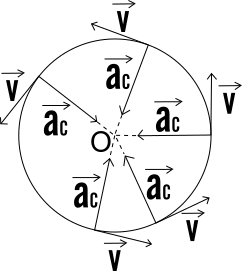
\includegraphics[scale=0.4]{moto-circolare-uniforme}
    \centering
    \caption{}
  \end{figure}

    \subsubsection{Periodicit\`a}
    È un moto periodico con periodo \(T = \frac{2 \pi R}{v} = \frac{2 \pi}{\omega}\), corrispondente al tempo necessario per compiere un giro completo.
    \subsubsection{Proiezione dei moti sugli assi cartesiani}
    I moti proiettati sugli assi cartesiani sono:
    \begin{align}
      x&= R \cos \theta = R \cos (\omega t + \omega_0) \\
      y&= R \sin \theta = R \sin (\omega t + \omega_0)
    \end{align}
	\subsection{Moto circolare non uniforme}
	Nel caso del moto circolare non uniforme si deve considerare l'accelerazione tangenziale $a_T=\frac{dv}{dt}$.
		\subsubsection{Accelerazione angolare}
		Essendo anche $\omega$ variabile si definisce l'accelerazione angolare:
		\begin{align*}
			a=\dfrac{d\omega}{dt}=\dfrac{d^2\theta}{dt^2}=\dfrac{1}{R}\dfrac{dv}{dt}=\dfrac{a_T}{R}
		\end{align*}
		\subsubsection{Determinare la velocit\`a angolare dall'accelerazione}
		Nota $a(t)$ si pu\`o integrare ottenendo:
		$$\omega(t)=\omega_0+\int_{t_0}^ta(t)dt$$
		$$\theta(t)=\theta_0+\int_{t_0}^t\omega(t)dt$$
		\subsubsection{Determinare l'incremento della velocit\`a angolare in corrispondenza dell'incremento angolare}
		Nota $a(\theta)$ si pu\`o calcolare l'incremento della velocit\`a angolare in corrispondenza all'incremento angolare $\theta-\theta_0$.
		\begin{align*}
			a&=\dfrac{d\omega}{dt}=\dfrac{d\omega}{d\theta}\dfrac{d\theta}{dt}=\\
			 &=\omega\dfrac{d\omega}{d\theta}\Rightarrow\\
			\Rightarrow&ad\theta=\omega d\omega\Rightarrow\\
			\Rightarrow&\int_{\theta_0}^\theta a(\theta)d\theta=\dfrac{1}{2}\omega^2-\dfrac{1}{2}\omega_0^2
		\end{align*}
		\subsubsection{Moto circolare uniformemente accelerato}
		Il moto circolare uniformemente accelerato \`e un moto in cui $a$ \`e costante, o $a_T$ costante.
		Ponendo $t_0=0$:
		$$\omega=\omega_0+at$$
		$$\theta=\theta_0+\omega_0t+\dfrac{1}{2}at^2$$
		L'accelerazione centripeta vale:
		$$a_N=\omega^2R=(\omega_0+at)^2R$$
		\subsubsection{Notazione vettoriale}
		Si ampli il concetto di velocit\`a angolare del moto circolare mostrando come si possono associare ad esso caratteristiche vettoriali.
		Si definisce velocit\`a angolare il vettore $\omega$ con modulo $\omega=\frac{d\theta}{dt}$, direzione perpendicolare al piano in cui giace la circonferenza e verso tale che all'estremo del vettore $\omega$ il moto appaia antiorario.
		Risulta evidente che:
		$$v=\omega\times r$$
		Nel caso $\omega$ sia applicata al centro della circonferenza $r=R$, ma questa equazione risulta valida se $\omega$ \`e applicata in un qualsiasi altro punto dell'asse di rotazione, ovvero la retta ortogonale al piano del moto e passante per il centro della circonferenza.
		Dato $\omega$ si individua l'asse di rotazione e il piano del moto circolare, il verso di percorrenza della circonferenza e come varia l'angolo nel tempo.
		Da $\omega$ per derivazione rispetto al tempo si ottiene il vettore accelerazione angolare $a$, parallelo a $\omega$ e verso determinato dalla variazione del modulo di $\omega$ e modulo $a=\frac{d\omega}{dt}$.
	\subsection{Accelerazione del moto circolare}
		Tramite $A$ e $\omega$ si esprime l'accelerazione del moto circolare:
		\begin{align*}
			a=\dfrac{dv}{dt}=\dfrac{d}{dt}(\omega\times r)=\dfrac{d\omega}{dt}\times r + \omega\times\dfrac{dr}{dt}\Rightarrow a=a\times r+\omega\times v
		\end{align*}
		Si nota come il primo termine $a\times r$ \`e l'accelerazione tangenziale $a_T$ di modulo $aR$, mentre il secondo $\omega\times v$ \`e l'accelerazione centripeta $a_N$ di modulo $\omega^2R$.
		Nel moto circolare uniforme $\omega$ \`e un vettore costante anche in modulo, $a$ \`e nulla e $a=a_N=\omega\times v$.
		\subsubsection{Propriet\`a di $r$}
		Il vettore $r$ applicato in $O$ ha modulo costante e descrive un moto rotatorio attorno all'asse di rotazione, ovvero alla direzione di $\omega$ formando un angolo $\phi$ costante con l'asse stesso.
		La sua derivata $\frac{dr}{dt}$ si pu\`o scrivere $\omega\times r$.
		Anche il vettore $v$ descrive una rotazione intorno a $\omega$ con cui forma l'angolo $\phi=\frac{\pi}{2}$ e la sua derivata $\frac{dv}{dt}$ si pu\`o scrivere $\omega\times v$.
		Al moto di rotazione di un asse rispetto ad un altro asse fisso con cui forma un angolo costante e ha un punto in comune si d\`a il nome di moto di precessione.
		Dato un vettore di modulo costante $A$ che descrive un moto di precessione con velocit\`a angolare $\omega$, la sua derivata temporale pu\`o essere sempre scritta:
		$$\dfrac{dA}{dt}=\omega\times A$$
		Che risulta ortogonale a $A$.
		Inoltre in modulo
		$$dA=A\sin\phi d\theta$$
		$$\dfrac{dA}{dt}=A\sin\phi\dfrac{d\theta}{dt}=\omega A\sin\phi=|\omega\times A|$$
\section{Moto parabolico dei corpi}
Si analizza il moto nel vuoto di un punto $P$ lanciato dall'origine $O$ con velocit\`a iniziale $v_0$ formante un angolo $\alpha$ con l'asse delle ascisse.
Si vuole calcolare la traiettoria, la massima altezza raggiunta e la posizione $G$ in cui il punto ricade su $x$ o la gittata $OG$.
	\subsection{Caratterizzazione}
	Il moto \`e caratterizzato da un'accelerazione costante $a=g=-gu_x$ e le condizioni inziali sono $r=0$ e $v=v_0$ al tempo $t=0$.
	Si nota come
	$$v(t)=v_0+\int_{t_0}^ta(t)dt=v_0-gtu_x$$
	\subsection{Velocit\`a}
	La velocit\`a si trova nel piano individuato dai vettori costanti $v_\theta$ e $g$, il piano $x,y$.
	Essendo $v_\theta=v_0\cos \alpha u_x+v_\theta\sin \alpha u_y$:
	$$v(t)=v_\theta\cos \alpha u_y+(v_\theta\sin \alpha-gt)u_x$$
	\subsection{Leggi orarie dei moti proiettati}
	La velocit\`a dei moti proiettati sugli assi sono $v_y=v_o\cos\alpha$ e $v_x=v_0\sin\alpha-gt$.
	Pertanto le leggi orarie dei moti proiettati sugli assi sono:
  \begin{multicols}{2}
    \noindent
    $$x=v_0\cos \alpha t$$
    $$y=v_0\sin\alpha t-\dfrac{1}{2}gt^2$$
  \end{multicols}
  \begin{tabular}{|p{13cm}}
	Se sull'asse $x$ il moto \`e uniforme, sull'asse $y$ \`e uniformemente accelerato.\\
  \end{tabular}
	\subsection{Traiettoria}
	La traiettoria viene ricavata eliminando il tempo tra $x(t)$ e $y(t)$ e ottenendo la funzione:
	$$y(t):t=\dfrac{x}{v_0}\cos\alpha$$
	$$y(x)=x\tan\alpha-\dfrac{g}{2v_0^2\cos^2\alpha}x^2$$
	Ovvero l'equazione di una parabola.
	\subsection{Direzione del moto}
	La direzione del moto in funzione del tempo o della coordinata $x$ pu\`o essere caratterizzata dall'angolo $\phi$ che il vettore velocit\`a forma con l'asse orizzontale:
	\begin{align*}
		\tan\phi=\dfrac{v_y}{v_x}=\tan\alpha-\dfrac{g}{v_0\cos\alpha}t=\tan\alpha-\dfrac{g}{v_0^2\cos^2\alpha}x
	\end{align*}
	Per calcolare la gittata $OG$ si impone $y(x)=0$ e si ottengono due soluzioni $x=0$ e:
	\begin{align*}
		x_G=\dfrac{2v_0^2\cos^2\alpha\tan\alpha}{g}=\dfrac{2v_0^2\cos\alpha\sin\alpha}{g}=2X_M
	\end{align*}
	Dove $X_M=v_0^2\frac{\cos\alpha\sin\alpha}{g}$ \`e la coordinata dal punto di mezzo del segmento $OG$ e ascissa del punto di massima altezza.
	\subsection{Altezza massima}
	L'altezza massima raggiunta \`e pertanto:
	$$y(X_M)=Y_M=\dfrac{v_0^2\sin^2\alpha}{2g}$$
	L'altezza massima si pu\`o ottenere annullando $\frac{dy}{dx}$, ovvero imponendo
	$$\tan\alpha-\left(\dfrac{g}{v_0^2}\cos^2\alpha\right)x=0$$
	Si ricava da questo l'ascissa del massimo $X_M$ e si calcola $y(X_M)$.
	Un altro modo \`e sfruttare il fatto che nel punto di massima altezza la velocit\`a \`e orizzontale, pertanto $u_y=0$ ovvero $t=t_M=v_0\sin\frac{\alpha}{g}$, sostituendo $x(t)$ e $y(t)$ si trovano $X_M$ e $Y_M$.
	\subsection{Angolo di lancio per la gittata massima}
	L'angolo di lancio per cui si ha la gittata massima si ottiene con la condizione $\frac{dx_G}{d\alpha}=0$ ovvero $\frac{2v_0^2}{g}(-\sin^2\alpha+\cos^2\alpha)=0$ e risulta $\alpha=45\si{\degree}$
	\subsection{Tempo totale di volo}
	Il tempo totale di volo $t_G$ \`e pari al tempo impiegato a percorrere $OG$ con velocit\`a costante $v_x=v_0\cos\alpha$:
	$$t_G=2\dfrac{X_M}{v_0}\cos\alpha=2v_0\sin\dfrac{\alpha}{g}=2t_M$$
	Si nota come $t_G$ coincide con il tempo necessario per salire a $Y_M$ e tornare al suolo.
	Si nota come nella posizione $G$ la velocit\`a \`e la stessa in modulo che alla partenza ma simmetricamente rispetto a $x$.
  \begin{multicols}{3}
    \noindent
    $$u_x(t_G)=v_0\cos\alpha$$
    $$u_y(t_G)=-v_o\sin\alpha$$
    $$\tan\phi=-\tan\alpha$$
  \end{multicols}

% \section{Riepilogo}
% \begin{itemize}
%   \item La descrizione del moto consiste nel determinare come varia la posizione del punto in funzione del tempo; se conosciamo la posizione ad un certo istante possiamo sapere come si sviluppa il moto se abbiamo la direzione istantanea del moto e la rapidità con cui avviene lo spostamento: ciò porta al concetto di velocità e possiamo concepire il moto come una successione di spostamenti infinitesimi \(d \overrightarrow{r}= \overrightarrow{v} dt\).
%   \item La velocità a sua volta può cambiare durante il moto e le sue variazioni sono espresse dall'accelerazione : \(d \overrightarrow{v} = \overrightarrow{\alpha} d t\).
%   \item La traiettoria è il luogo dei punti occupati in funzione del tempo dalla punta del vettore \(\overrightarrow{r}(t)\): questo dà la posizione del punto, ma non la direzione del moto espressa, come detto sopra, da \(d \overrightarrow{r}\) e quindi da \(\overrightarrow{v}\).
%   \item La velocità v è dunque sempre tangente alla traiettoria; l'accelerazione in generale non è parallela alla velocità. La componente di \(\overrightarrow{\alpha}\) ortogonale a \(\overrightarrow{v}\) descrive le variazioni della direzione del moto e non ha alcun legame con le variazioni del modulo di \(\overrightarrow{v}\). Nel moto curvilineo c'è sempre una componente dell'accelerazione ortogonale alla traiettoria, nel moto rettilineo questa componente è sempre nulla.
%   \item Da \(r(t)\) si passa a \(\boldsymbol{v}(t)\) e ad \(\boldsymbol{a}(t)\) derivando rispetto al tempo; se invece è data \(\boldsymbol{a}(t)\) il passaggio inverso si fa integrando ed è essenziale la conoscenza delle condizioni iniziali.
%   \item Le grandezze cinematiche fondamentali sono dunque posizione, velocità, accelerazione e sono legate tra loro da operazioni di derivazione e di integrazione, conseguenza del fatto che lo studio dell'evoluzione del moto comporta il concetto di variazione che è espresso matematicamente dall'operazione di derivazione.
%   \item \(\mathbf{r}, \boldsymbol{v}, \boldsymbol{a}\) sono grandezze vettoriali: nella loro definizione oltre ad un numero bisogna dare una direzione e un verso; pertanto le variazioni di posizione e di velocità sono espresse completamente solo se si tiene conto sia della variazione del modulo che della variazione della direzione.
%   \item È necessario specificare sempre in quale sistema di riferimento si descrive il moto: le coordinate del punto, le componenti di \(\boldsymbol{v}\) e \(\boldsymbol{a}\), l'espressione analitica della traiettoria dipendono dal sistema di riferimento. Però le relazioni più generali tra le grandezze cinematiche sono relazioni vettoriali e in quanto tali sono invarianti rispetto alla scelta del sistema di riferimento, cioè valgono in qualsiasi sistema di riferimento.
%   Quindi, se \(\mathbf{b}=\mathbf{c}\), questo comporta sempre \(b_{x}=c_{x}, b_{y}=c_{y}, b_{z}=c_{z}\) ma i valori \(\left(b_{x}, b_{y}, b_{z}\right)\) e \(\left(c_{x}, c_{y}, c_{z}\right)\) cambiano col sistema di riferimento.
% \end{itemize}

\end{document}
